\begin{figure*}[htbp]
\centering
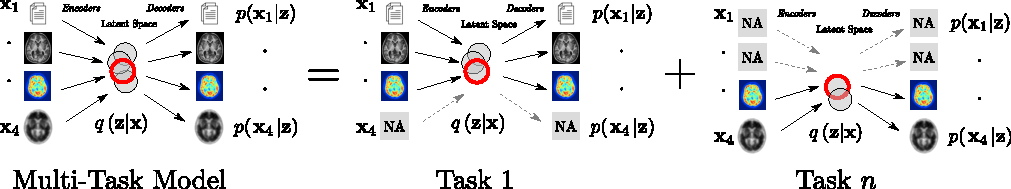
\includegraphics[width=\textwidth]{./tex/fig/model.pdf}
\caption{
Simple example of a Multi-Task Model learning scheme in the presence of missing not available (NA) views.
Arrows represent learnable functions used as network encoders and decoders, transforming respectively input views (\eg clinical scores, imaging derived phenotypes, \ldots) from the observation space to the representation space (circles) and from the representation space back to the observation space.
The separability of the loss function $\LBdnv$ in \eqnref{eq:newLB} allows to group together observations into homogeneous learning tasks.
For every task, functions associated to missing views (dashed gray arrows) are locally not updated by the learning algorithm.
Globally, common latent representations (red circles) across pairs of tasks act as a link allowing the information to flow throughout the views.
}
\label{fig:model}
\end{figure*}
